% ----------------------------------------------------------------------------------------
% CHAPTER TITLE
% ----------------------------------------------------------------------------------------
\chapter{A History of Post-Optimal Objects in Electronic Music}\label{background}
\lhead{\chaptertitlename\ \thechapter. \emph{Background}}
% ----------------------------------------------------------------------------------------

Great effort goes into making commercial electronics consistent, predictable and uniform regardless of inconsistencies in parts values. The same largely holds for industrially marketed electronic instruments: ``one-offs" with unpredictable behaviors or cryptic functions drastically reduce overall adoption of the device, and therefore, their commercial potential \cite[p.5]{haslett2005}. In this context, the gap between the determinism of product design and the desire for originality of musical performances is bridged by the musician. ``Finding your sound" is about finding an instrument and using it effectively.  

Making, modifying or otherwise altering electronics is one option to better understand the tools at a musician's disposal and make the most of them. In order to better understand what shaped Buchla's and Collins' work, this chapter draws a brief history of musical electronics that serves as a background for contemporary case-studies presented in the following section.

\section{Electronic Music as Invention}

Electronic music was invented before it was composed. Relying on a spirit of curiosity and experimentalism dear to later figures such as Tudor, Collins or Ghazala, pioneers such as C.G. Page, Elisha Gray or Thaddeus Cahill developed electronic musical systems for no reason other than curiosity. As their inventions (galvanic music, the musical telegraph, the Telharmonium) failed to be scientific or financial successes, they abandoned these alleys of research, unaware of their successors' importance \citep{page1837,nasmyth1908,holmes2002}. 

With electronics still in infancy - no design tradition, few formal structures - blind experimentation was the only option. As design methodologies such as the kit of parts had not been imagined, these devices are not \textit{post-optimal}. However, they do offer a glimpse at  electronic music when it was a matter of invention rather than composition. 

Two major exceptions were notable for their financial, musical and technical successes: Edison's Phonograph and Termen's Theremin.  
		
Edison was an accomplished inventor and astute investor \citep{collins1998}. The phonograph he toured to advertise in 1877 emphasized the intelligibility of the voices it reproduced. Although critics pointed out the impressive but imperfect output from the device, Edison maintained that audiences couldn't accurately distinguish his mechanized reproduction from the natural voice, offering demonstrations tours across the United States \citep{thompson1995}. The phonograph is the first example of optimal audio device, one which achieves usability but understates its creative potential \citep{collins1998}. 
	
In turn, the Theremin (1920) and its relative financial, but also musical and technical successes presents a significant complement to the phonograph. Just like the Telharmonium, the Theremin can produce some familiar sounds, but with a much simpler device:  

\begin{figure}[H]
	\centering
	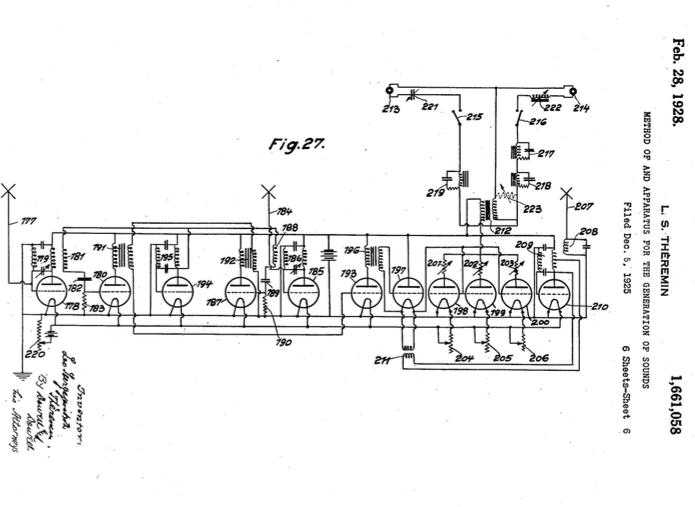
\includegraphics[width=1\textwidth]
	{theremin}
	\caption{The Theremin's complete schematic \citep[p.6 of 17]{theremin1928}}
\end{figure} 

Compare this with even just one of the Telharmonium's tone generating electromechanical systems: 

\begin{figure}[H]
	\centering
	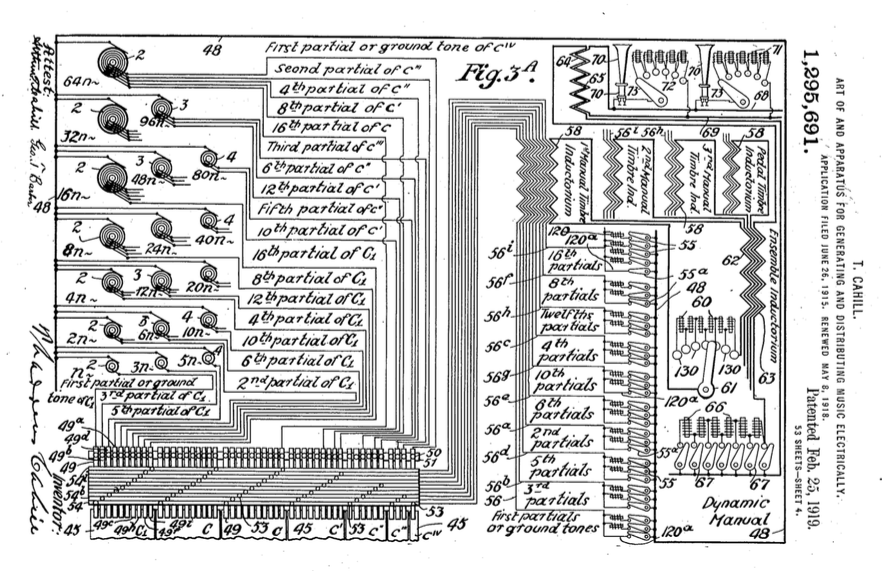
\includegraphics[width=1\textwidth]
	{telharmonium}
	\caption{The Telharmonium's tone generating electro-mechanical circuit \citep[p.4 of 141]{cahill1919}}
\end{figure} 

The Theremin's elegant simplicity is related to the hazardous nature of its discovery, best resumed by Kock: 

\begin{quote}
 The early home-made vacuum tube sets, particularly those called "super-heterodyne sets," often possessed the annoying habit of suddenly emitting a loud squeal from the loudspeaker, causing the embarrassed young designer to leap immediately toward the set to readjust the tuning and thereby stop the squeal. In the process of his approaching the set, the nearness of his body introduced a (capacitive) electrical effect which caused the pitch of the squeal to change, going either to a higher-pitched tone or to a lower-pitched one.
\end{quote}

\citep[p.33]{kock1978}

The theremin, like Gray's musical telegraph, is a by-product of scientific research. However, it comes at a time where its base components are publicly available, backed by population-wide interest in radio technologies and the economic incentive to build electronics from kits. In effect, the theremin embodies a shift in electronic music from component innovation to systems and interface innovation, which make designs commercially and compositionally viable. 

\section{Electronic Music as an Institutional Practice}

This shift is, as hinted above, mostly enabled by world-war era research and manufacturing \citep[p.81]{holmes2002}, especially the vacuum tube triode. 

As design methods for vacuum tube-based circuits developed, schematic and tools were thoroughly investigated, optimized and standardized. Building off their industrial successes, institutions served as the breeding ground for most renowned artistic applications of technology: the emergence of the French (ORTF), German (WDR), and Italian (RAI) experimental music studios is directly linked to the increasing popularity of public radio stations. In the U.S., RCA and Columbia University composers collaborated to develop the RCA synthesizer \citep{holmes2002}. Max Matthews, after being trained as a Navy radio repairman, found work at Bell Labs with music enthusiast John Pierce, whose fostering would mark the beginning of computer music \citep{park2009}.

	\begin{figure}[H]
	  \centering
	    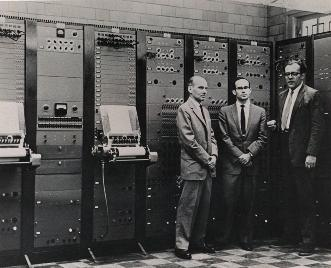
\includegraphics[width=1\textwidth]{rcamkii}
	     \caption{The RCA Mk.II with Milton Babbitt, Peter Mauzey, Vladimir Ussachevsky, 1958}
	\end{figure}  
	
Those state-funded studios or private research departments constructed a framework for electronic music composition, based on additive / subtractive synthesis techniques and tape editing. But even in those still rigid environments, alternative approaches to instrument design emerged:  In Canada, Hugh Le Caine left nuclear physics research to develop the Electronic Sackbut. His device implemented both early version of voltage control and semi-autonomous composition starting in 1945 \citep{holmes2002}. The Sackbut's unpredictable response to left-hand controls place its interface squarely in the domain of post-optimal objects. 

\begin{figure}[H]
	  	  \centering
	    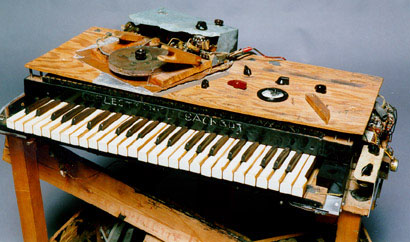
\includegraphics[width=1\textwidth]{sackbut}
	    \caption{The Electronic Sackbut by Hugh LeCaine}
	\end{figure}

In parallel, high costs of manufactured electronics between the world wars kickstarts the birth of do it yourself (DIY) culture. In 1922, a Freshman “masterpiece” radio cost \$17 as a kit, while a completed set cost \$60. This corresponds to \$240 v. \$850 in 2014 \citep{radioblvd2014, data.blgs.gov2014}. Accordingly, Radio Shack’s first catalog  from 1939, contained 80\% kits, parts and tools and 20\% completed products. A significant number of young engineers growing up with this democratization of technology bring electronic music outside of large institutions. These engineers would echo Le Caine's work, embracing ideals of inconsistent interfaces, intuitive circuit design, and autonomous systems. 

One such engineer was Raymond Scott, a professional film composer. He assembled  some of the first incarnations of multi-track tape recorders and self-composing synthesizers: his Electronium is described as an instrument that could only be influenced by the user \citep[p.142]{holmes2002}. ``...the Electronium adds to the composer's thoughts, and a duet relationship is set up between man and machine'' \citep{chusid1999}. The Electronium ``is not played, it is guided''\citep{darter1984}. Again, a unique approach to interface design places the device within the realm of post-optimal objects.  

	\begin{figure}[H]
	  \centering
	    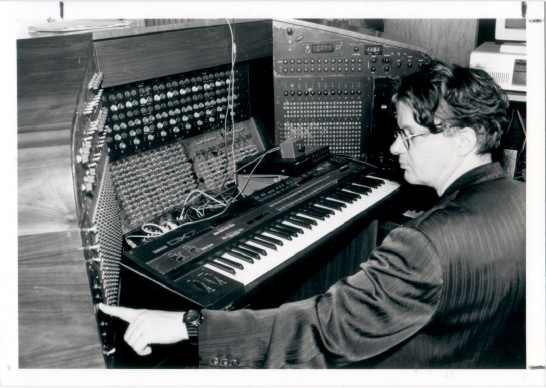
\includegraphics[width=1\textwidth]{electronium}
	     \caption{The Electronium by Raymond Scott, with Mark Mothersbaugh, its current owner, 1993}
	\end{figure}

Finally, John Cage collaborators Louis and Bébé Barron were arguably the most compelling example of post-optimal musical electronics up to this point. Their use of  cybernetics model developed by Norbert Wiener \citep{wiener1965} as basis for musical devices would prove to be yet another early example of a trend, but their hardware implementation was truly unique up to this point: the circuits that Louis built were poorly designed, overdriven and eventually, failed. They would describe the resulting devices as ``alive'' \citep{barron2009}. These decaying sound processes would be used as the basis for their composition, which they assembled in a way similar to Schaeffer’s concrète process \citep{dunbar2010}.

	\begin{figure}[H]
	  \caption{Louis and Bébé Barron in the studio}
	  \centering
	    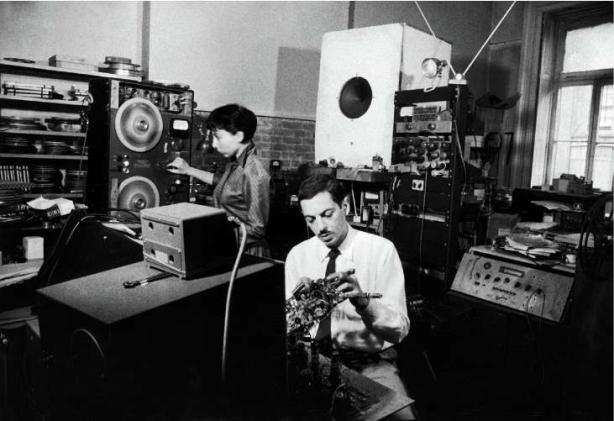
\includegraphics[width=1\textwidth]{barrons}
	\end{figure} 
	
The Barron's devices are perhaps the most compelling proof that personalized musical instruments with post-optimal traits were accessible to those outside of academia and private research.

If the simultaneous rise of vacuum tubes and the theremin allowed electronic music to slowly enter the popular subconscious, it is designers like LeCaine, Scott and the Barron that lead the way in suggesting that hardware wasn't exclusively the domain of the professional engineer. In their design, post-optimal systems and interfaces are a clear, albeit under-documented, thread. This thread comes to full light with the next technological advancement, solid state technologies. 

\section{Electronic Music as Living Systems}

The development of the silicon transistor, invented in 1947 and commercialized in 1954 \citep{texasinstrument}, effectively brought down the last barriers for composers to engage directly with the tools that allowed them to make electronic music: price, reliability and safety.  

\begin{figure}[H]
    \centering
    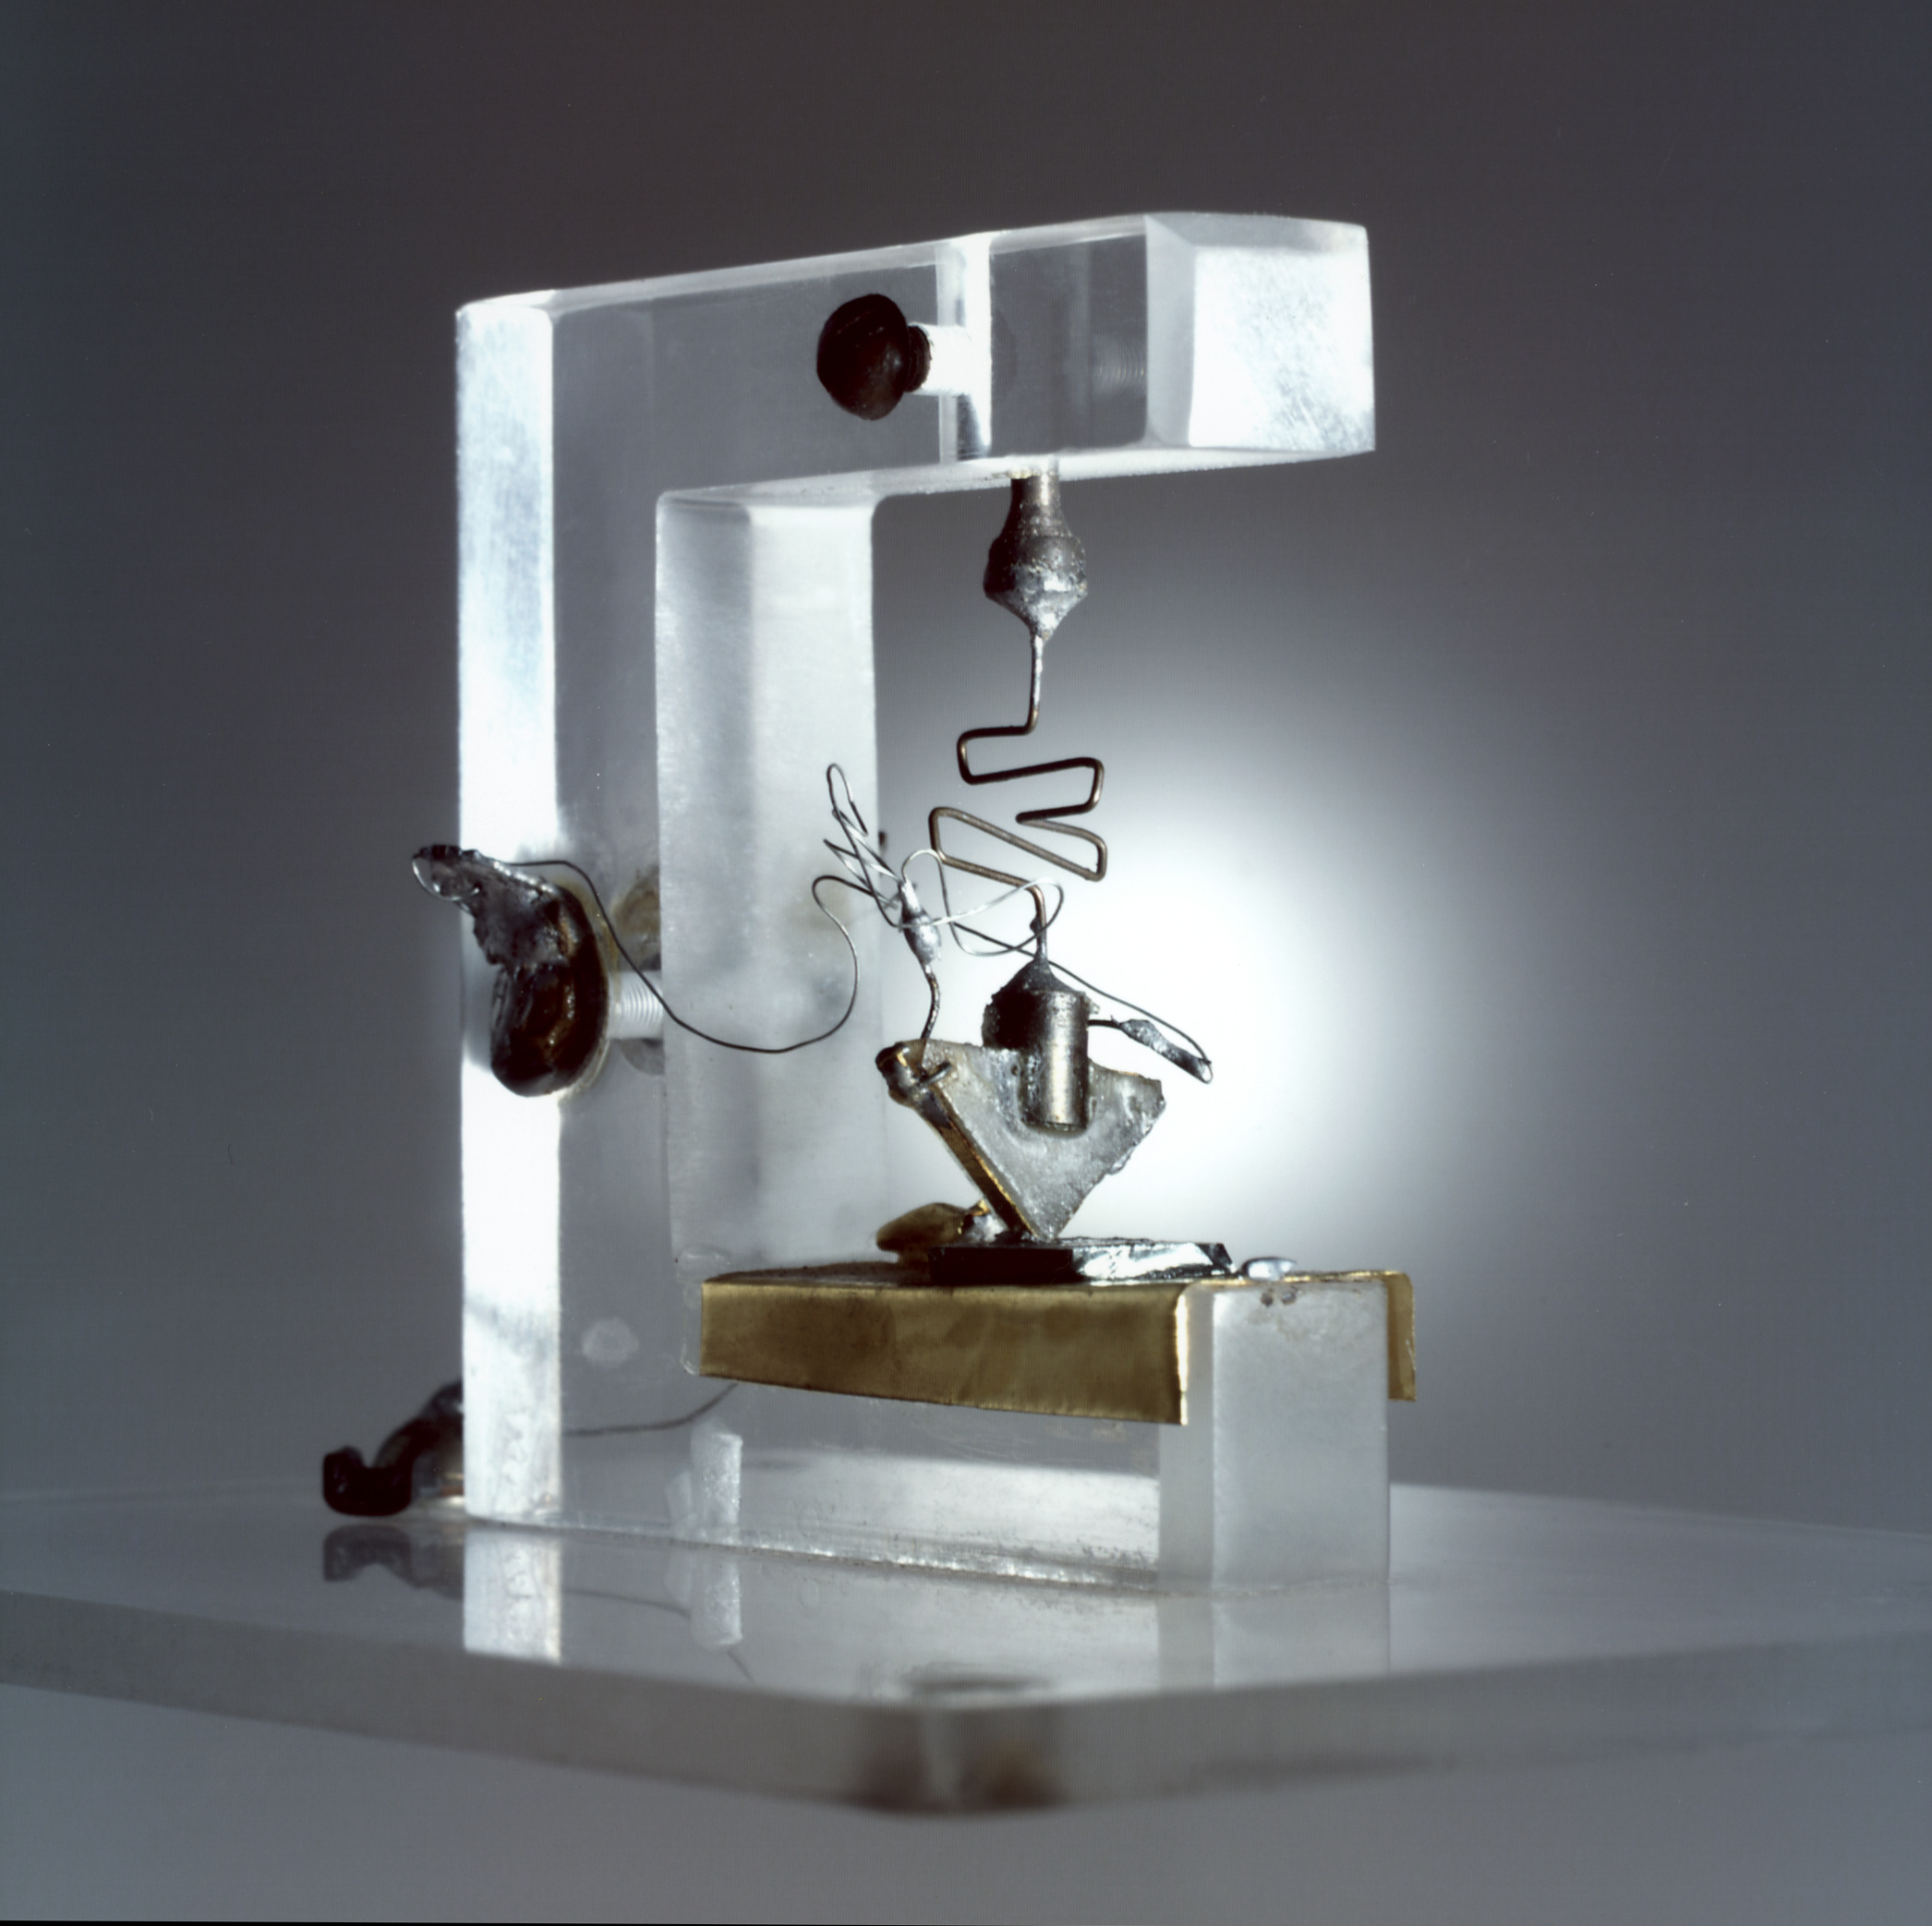
\includegraphics[width=.5\textwidth]{transistor}
    \caption{The first functional transistor, Bell Laboratories, 1947 (replica)}
\end{figure}

\subsection{Voltage Control}

Robert Moog, Donald Buchla and Serge Tcherepnin are all examples of engineers building off their experience with kits and lifelong interests in electronics to fully realize the musical promises of solid-state technologies. The result is an expensive but publicly available package: the modular synthesizer. As those designers were products of institutions (Buchla worked at NASA, Moog at Cornell University, Tcherepnin in Cologne and CalArts), these synthesis systems mirrored the additive and subtractive methodologies developed by the likes of Babbitt, Ussachevsky and LeCaine. However, they did so in relatively compact formats that allowed for very wide variation and versatility. The parallel with academic computer music is straightforward: unit generators are the equivalents of voltage control oscillators (VC0) and their low frequency equivalents (LFO), ring modulation is multiplication, add/substract units are mixers, etc. 

One can see in the commercial modular synthesizer as a first opportunity for the public to ``build'' personalized systems for popular music. Although modules are limited and costly, the end user is responsible for the final layout of their device. 

	\begin{figure}[H]
	  \centering
	    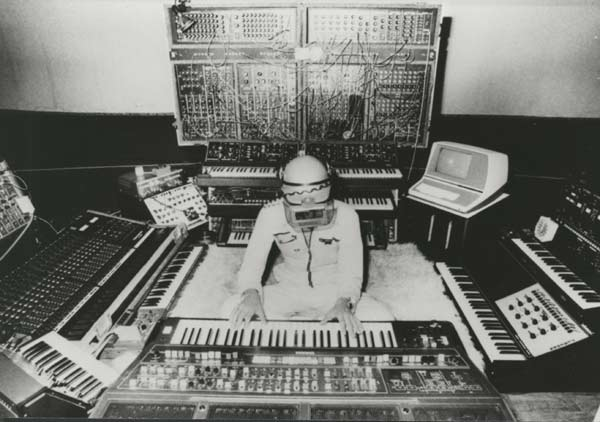
\includegraphics[width=1\textwidth]{schulze}
	    \caption{The Big Moog Modular System with Klaus Schulze, mid 1970's}
	\end{figure}

Although Moog is not the only manufacturer of modular systems, his choice to pair his devices with the more musically familiar keyboard and some public relations skills make him the bridge between classical tape and electronic composers. What Wendy Carlos sees as the tools of ``ugly music'' can now be used for ``appealing music you could listen to.'' \cite[p.169]{holmes2002} As Carlos fine-tuned her own Moog system, she eventually went to get a custom version of the system made to her specifications and make electronic music exponentially more popular through her \textit{Switched On Bach} record. 

	\begin{figure}[H]
	  \centering
	    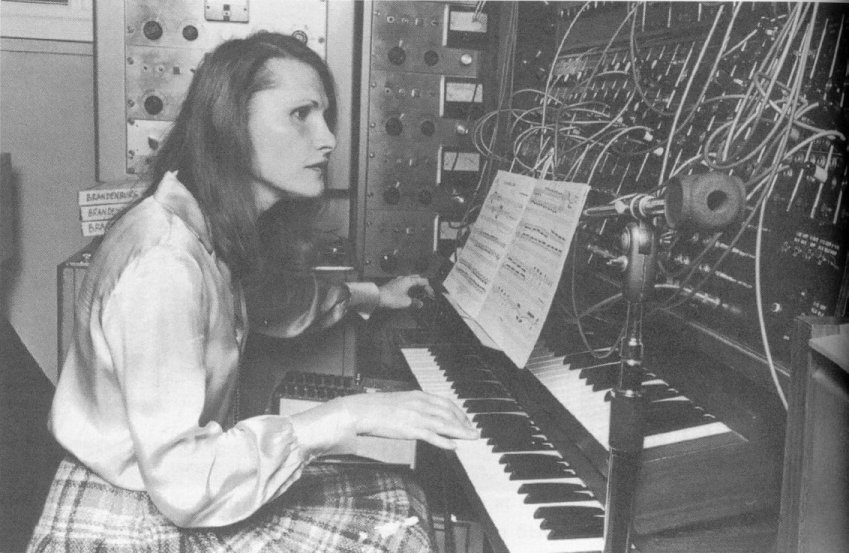
\includegraphics[width=1\textwidth]{carlos}
	    \caption{The Moog 55 system customized for Wendy Carlos}
	\end{figure}

At the opposite end, Buchla viewed himself as a luthier, designer of instruments, rather than the engineer of machines \citep{pinch2001}. His decision to develop new methods of interacting with his circuitry rather than relying on pre-existing schemes like Moog's keyboard severely limited his user-base. Nevertheless, Buchla's designs are respected and still popular today: ``The Buchla box was designed for musicians who wanted to produce a complex piece of music in real time.'' \citep[p47]{pinch2002}. If Moog's modular model is the template for much of the additive synthesis audio software and hybrid analog/digital audio hardware today, Buchla's interface and interactive system design work are still being digested and re-used \citep{rylan2015,snyder2012} . 

	\begin{figure}[H]
	  \centering
	    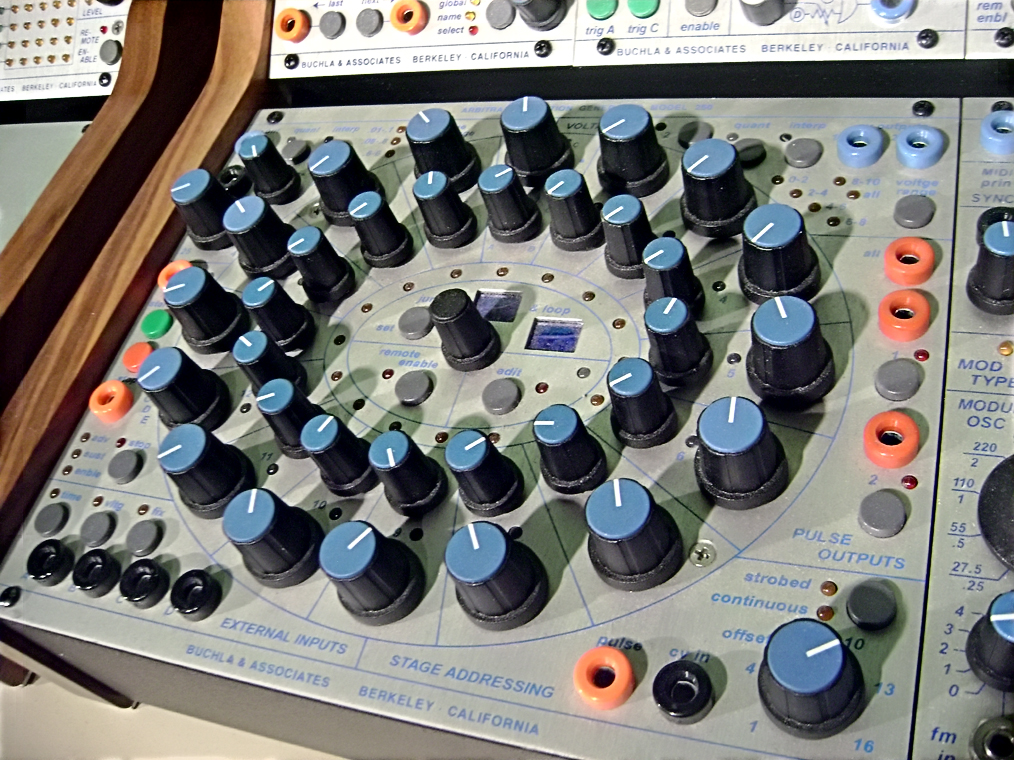
\includegraphics[width=1\textwidth]{buchlaarb}
	     \caption{The Arbitrary Function Generator, Buchla's distinctive aleatory module}
	\end{figure}

Ultimately, Pinch concludes: ``Designers `script' or `configure' ideal users into their machines.(...) Scripts try to contain the agency of users, but users can exert agency, too, and can come up with their own alternative scripts." \cite[p.311]{pinch2002}. The complex interplay between designer and user takes on a significantly different meaning when those two personas belong to the same person. In that sense, being both the designer of the system and the user allows for post-optimal objects to emerge.
	
As engineers like Moog and Buchla abandoned their institutional positions to develop these modular systems, the American experimental music scene was also enjoying unprecedented exposure. Of interest here is David Tudor, and a major turning point was his performance of Cage's 1961 \textit{Variations II}. 

\subsection{Composers Inside Electronics}

Preparing the piece, Tudor assembled a complex electronic system which continually produced musical signals. Control on the system was tenuous at best: “You could only hope to influence the instrument” \citep{nakai2014}. 
	 
 	\begin{figure}[H]
 	  \centering
 	    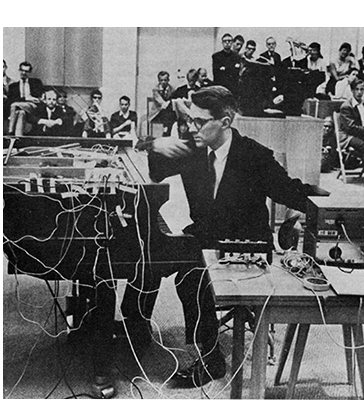
\includegraphics[width=1\textwidth]{tudorvar}
 	    \caption{Variations II, performed by Tudor}
 	\end{figure}
	
Tudor would go on to build a composition career based largely on this premise of live electronics. Reminiscent of Barron’s living circuits, Tudor described his work as “composing itself out of its own composite instrumental nature.”\citep{tudor,kuivila2004} Tudor's practice of experimental electronic music systems complements Cage’s indeterminacy, and this was made possible because of semiconductors (Collins, Appendix A). Transistors and integrated circuits offered the functionality of vacuum tubes without the latter’s size, weight, price and high voltage hazards, becoming available and documented as he started using custom electronics \citep{collins2004}. Tudor elaborates: 

\begin{quote}
						
Electronic components and circuitry, observed as individual and unique rather than as servomechanisms, more and more reveal their personalities, directly related to the particular musician involved with them. The deeper this process of observation, the more the components seem to require and suggest their own musical ideas, arriving at that point of discovery, always incredible, where music is revealed from ``inside,'' rather than from ``outside.'' 

\end{quote}

\citep{tudor1976,nakai2014}

Furthermore, Tudor is arguably unique for being the first to so explicitly bridge \textit{poetic} visions of circuits and composition with a complementary approach to musical scores:   

\begin{figure}[H]
	  \centering
	    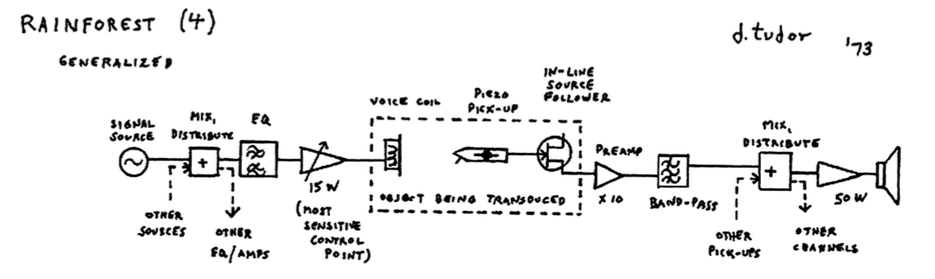
\includegraphics[width=1\textwidth]{rainforest4}
	    \caption{The score for \emph{Rainforest IV} by David Tudor}
	\end{figure}

	\begin{figure}[H]
	  \centering
	    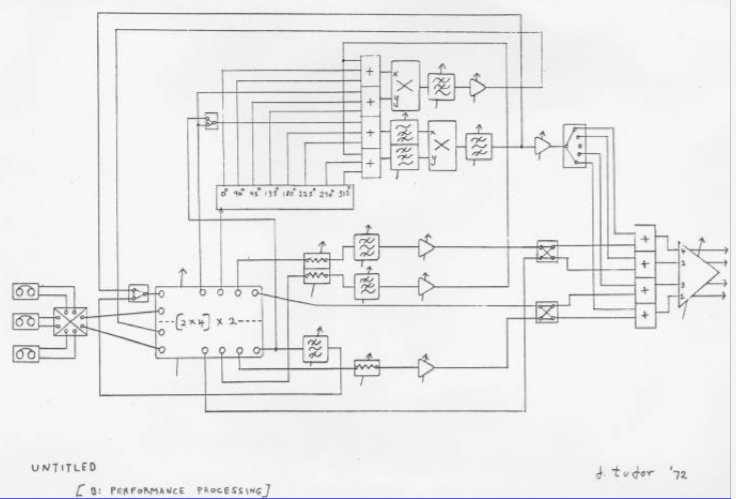
\includegraphics[width=1\textwidth]{untitled}
	      \caption{The score for \emph{Untitled} by David Tudor}
	\end{figure}
	
These take a formalized practice of abstraction (the circuit schematic), and push it one step further through unusual variations relating to personal interpretations rather than an universal symbology. Graphic scores were by then not an original practice, however, few offered such a clear connection between the musical and physical realities of the compositions.

Both aspects of Tudor's practice can be considered as post-optimal: his circuits behaved as co-composers through complex, unpredictable and sometimes chaotic operations (those systems are still rarely used in standard electrical engineering today), and his schematic-scores challenged the performer to produce personal interpretations of these twice-abstracted symbol combinations. 

These innovative methods were largely a collaborative practice. Through collaborations with Gordon Mumma, David Behrman, Hugh Le Caine, or John Fulleman and thorough personal investigation, he gathered enough experience to masterfully implement one of the first documented uses of chaotic electronics in music \citep{kuivila2004}. Some of these collaborations (namely with John Driscoll, Paul DeMarinis, Nicolas Collins, Matt Rogalsky, Ron Kuivila, amongst many) were formalized as \textit{Composers Inside Electronics} (CIE) for the premiere of \textit{Rainforest IV} in 1973. Tudor and his students shaped live electronic music performance \citep{collins2004,collins2006,collins2008,collins2010,nakai2014,driscoll2004,kuivila2004}. Through the learning, supplying and sharing tools offered online, Tudor’s ideals of experimentation and collaboration have come to be more relevant and accessible than ever.   

A prime example of avant-garde, personal electronic music techniques coming to a popular forefront with relatively little technical support comes from the British composer Brian Eno, through his development of the system later known as \emph{Frippertronics}. His process on \emph{Discreet Music} is clearly related to Tudor's: 

\begin{quote}
	If there is any score for the piece, it must be the operational diagram of the particular apparatus I used for its production. \citep{eno1975}
\end{quote}

\begin{figure}[H]
  
  \centering
    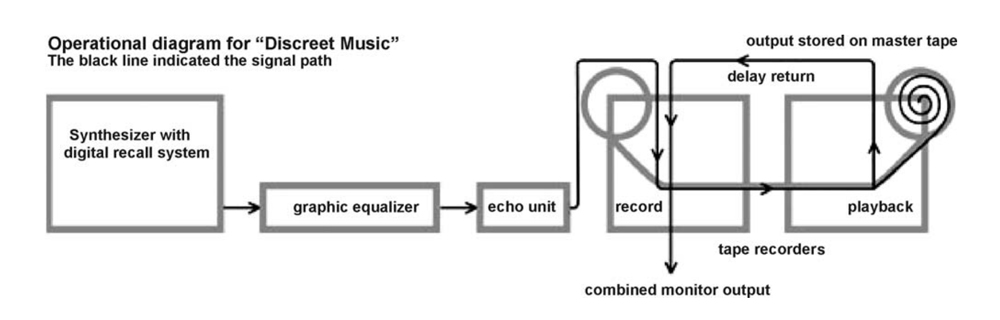
\includegraphics[width=1\textwidth]{discreetdiagram}
    \caption{The Operational Diagram for Discreet Music\citep{eno1975}}
\end{figure}

In terms of post-optimal approaches, Eno operates between the system and interaction levels. However, Tudor's wish to see personality emerge from circuits is echoed by Eno's  ``acceptation of that passive role'' which characterizes the first half of \emph{Discreet Music}. 

More so than Tudor's various devices, \emph{Frippertronics} serve as the archetype of simple post-optimal electronic music instruments. It illustrates the amount of resources, technical knowledge and musical intuition necessary to make the medium of electronic music one's own. Tudor and Eno, by using diagrams as scores rather than standard staff notation, redefine the notion of musical literacy and expertise. 

\section{Electronic Music as Craft: Silicon Luthiers} 

Academically, the essence of Tudor’s successors’ would be captured by CIE member Nicolas Collins:

\begin{quote}
“The circuit— whether built from scratch, a customized commercial device, or store-bought and scrutinized to death— became the score.”
\end{quote}

\citep{collins2004}

\emph{Handmade Electronic Music} was first published in 2006, presenting an extensive amount of information on homemade electronic instruments with insight from years of experience, references and sources. By completing this project, Collins not only proved that blending academic, commercial and hobbyists attitudes could be successful in all three of those areas, but also linked decades of practices in the do-it-yourself electronic music world to the “maker” movement. 

Discussing Tudor, Mumma and Kahn, Collins describes the origin of his interest in music hacking, which references the origin of experimental electronics as a legitimate ground for musical composition: 

\begin{quote}
“I learned from Tudor and Mumma that you did not have to have an engineering degree to build transistorized music circuits. David Tudor’s amazing music was based partly on circuits he did not even understand. He liked the sounds they made, and that was enough.” 
- David Berhman \cite[p.ix]{collins2006}  
\end{quote}

In effect, \textit{Handmade Electronic Music} is a manual for the design, manufacture and refinement of post-optimal musical electronics, starting at the component level and working to larger systems. Collins gives an informal list of the ``unsung heroes'' of this practice: Moog, Buchla, Tcherepnin, but also Tom Oberheim, Alan Pearlman, Craig Anderton and David Cockerell, then followed more recently by Bob Bielecki, Bert Bongers, and Sukandar Katardinata \citep[p.211]{collins2006}. Those are later named  \textit{Silicon Luthiers}: they are, in effect, the master craftsmen of electronic music instruments \citep{collins2008}.

Just like Tudor and Lucier helped younger practitioners develop their own hardware based approach, Collins' book encourages an inclusive and intuitive vision of tinkering and experimentation for the arts, and does so through more than a friendly informal tone. The original draft for the book, a compilation of class notes, is freely available for download off of the author’s website \citep{collins} . The first result for “handmade electronic music pdf” on most search engines will give a pdf of book.

By tolerating or passively encouraging open access to resources, Collins gives back directly to the community he has helped shape. More than writing the book on hardware hacking for non-engineers, he’s an essential force in making open hardware design the self-sustaining cycle it aspires to be through the maker movement. By publishing this through a large company while in a professional academic and musical position, he also lends the weight of a more widely recognizable figure to a movement and methodology that challenges the necessity for those very institutions.

Measuring the influence of this book through simple academic metrics, such as the number of times it is cited in publications following it \citep{harzing2008} yields the following results. “Handmade…” seems to have been referenced in 88 publications. For comparison, Road’s “Computer Music Tutorial”, published 10 years earlier, returns 1267 citations, the “Art of Electronics” (a standard circuit design text from 1989) returns 3640, and Gharzala’s “Circuit Bending” from 2005 returns 45. 

When it is cited, “Handmade…” is rarely commented upon directly. It is referred to in surveys of contemporary sound art, music, and music technology practices \citep{kelly2011,mills2010,pigott2011,rodgers2010}, and as an inspiration in the development of a specific musical controller \citep{ariza2007,hoadley2010,murphy2010,riis2013,valle2011}.
	
Overall, the academic impact of the work is fairly confined to the field it wished to solidify (music hardware hacking). Its varied content originated from a set of lecture notes, which have since found their place in other college level classes at other institutions. 

On a community level, Collins’ impact is difficult to measure objectively. Highly frequented music hardware hacking forums such as Experimentalist Anonymous, DIYstompboxes, freestompboxes.org, and electro-music.com all contain mention and praises for the accessibility and simplicity of “Handmade…”, but those explicit references are rare. For comparison, searching for Ray Wilson’s popular “music from outer space” do-it-yourself synthesizer website returns between two to three times more results on the same forums. However, as the upcoming case-studies will indicate, Collins' writing has had a long-lasting practical effect on music tinkerers. Further publications prove that although Collins' text is not the only resource available, he has contributed to the development of entire sub-genres of musical expression based entirely on explorations of audio hardware hacking \citep{ghazala2004,hegarty2007,kelly2009}. 

\newpage

This history elucidated how Dunne's concept of post-optimality could link seemingly disparate practices in the design and fabrication of musical instruments: first, inventors' curiosity to combine the new medium of electricity with the older purpose of music helped define what metrics the greater engineering community would use to determine optimal objects. Second, the advent of vacuum tubes and solid state technologies empowered growing waves of tinkerers to apply knowledge and research from radio communications and explore possibilities outside of what best practices recommended, slowly offering an alternative to the institutional practice of electronic music. Finally, these post-optimal practices were legitimized by academics in order to further disassociate an engineering backgrounds from the design electronic music instruments. 

This leads this discussion to the current state of post-optimal objects in electronic music: what drives practitioners to implement such approaches, and what advantages might they still offer? 

% ---------------

